\documentclass[twoside]{book}

% Packages required by doxygen
\usepackage{fixltx2e}
\usepackage{calc}
\usepackage{doxygen}
\usepackage[export]{adjustbox} % also loads graphicx
\usepackage{graphicx}
\usepackage[utf8]{inputenc}
\usepackage{makeidx}
\usepackage{multicol}
\usepackage{multirow}
\PassOptionsToPackage{warn}{textcomp}
\usepackage{textcomp}
\usepackage[nointegrals]{wasysym}
\usepackage[table]{xcolor}

% Font selection
\usepackage[T1]{fontenc}
\usepackage[scaled=.90]{helvet}
\usepackage{courier}
\usepackage{amssymb}
\usepackage{sectsty}
\renewcommand{\familydefault}{\sfdefault}
\allsectionsfont{%
  \fontseries{bc}\selectfont%
  \color{darkgray}%
}
\renewcommand{\DoxyLabelFont}{%
  \fontseries{bc}\selectfont%
  \color{darkgray}%
}
\newcommand{\+}{\discretionary{\mbox{\scriptsize$\hookleftarrow$}}{}{}}

% Page & text layout
\usepackage{geometry}
\geometry{%
  a4paper,%
  top=2.5cm,%
  bottom=2.5cm,%
  left=2.5cm,%
  right=2.5cm%
}
\tolerance=750
\hfuzz=15pt
\hbadness=750
\setlength{\emergencystretch}{15pt}
\setlength{\parindent}{0cm}
\setlength{\parskip}{3ex plus 2ex minus 2ex}
\makeatletter
\renewcommand{\paragraph}{%
  \@startsection{paragraph}{4}{0ex}{-1.0ex}{1.0ex}{%
    \normalfont\normalsize\bfseries\SS@parafont%
  }%
}
\renewcommand{\subparagraph}{%
  \@startsection{subparagraph}{5}{0ex}{-1.0ex}{1.0ex}{%
    \normalfont\normalsize\bfseries\SS@subparafont%
  }%
}
\makeatother

% Headers & footers
\usepackage{fancyhdr}
\pagestyle{fancyplain}
\fancyhead[LE]{\fancyplain{}{\bfseries\thepage}}
\fancyhead[CE]{\fancyplain{}{}}
\fancyhead[RE]{\fancyplain{}{\bfseries\leftmark}}
\fancyhead[LO]{\fancyplain{}{\bfseries\rightmark}}
\fancyhead[CO]{\fancyplain{}{}}
\fancyhead[RO]{\fancyplain{}{\bfseries\thepage}}
\fancyfoot[LE]{\fancyplain{}{}}
\fancyfoot[CE]{\fancyplain{}{}}
\fancyfoot[RE]{\fancyplain{}{\bfseries\scriptsize Generated by Doxygen }}
\fancyfoot[LO]{\fancyplain{}{\bfseries\scriptsize Generated by Doxygen }}
\fancyfoot[CO]{\fancyplain{}{}}
\fancyfoot[RO]{\fancyplain{}{}}
\renewcommand{\footrulewidth}{0.4pt}
\renewcommand{\chaptermark}[1]{%
  \markboth{#1}{}%
}
\renewcommand{\sectionmark}[1]{%
  \markright{\thesection\ #1}%
}

% Indices & bibliography
\usepackage{natbib}
\usepackage[titles]{tocloft}
\setcounter{tocdepth}{3}
\setcounter{secnumdepth}{5}
\makeindex

% Hyperlinks (required, but should be loaded last)
\usepackage{ifpdf}
\ifpdf
  \usepackage[pdftex,pagebackref=true]{hyperref}
\else
  \usepackage[ps2pdf,pagebackref=true]{hyperref}
\fi
\hypersetup{%
  colorlinks=true,%
  linkcolor=blue,%
  citecolor=blue,%
  unicode%
}

% Custom commands
\newcommand{\clearemptydoublepage}{%
  \newpage{\pagestyle{empty}\cleardoublepage}%
}

\usepackage{caption}
\captionsetup{labelsep=space,justification=centering,font={bf},singlelinecheck=off,skip=4pt,position=top}

%===== C O N T E N T S =====

\begin{document}

% Titlepage & ToC
\hypersetup{pageanchor=false,
             bookmarksnumbered=true,
             pdfencoding=unicode
            }
\pagenumbering{roman}
\begin{titlepage}
\vspace*{7cm}
\begin{center}%
{\Large My Project }\\
\vspace*{1cm}
{\large Generated by Doxygen 1.8.11}\\
\end{center}
\end{titlepage}
\clearemptydoublepage
\tableofcontents
\clearemptydoublepage
\pagenumbering{arabic}
\hypersetup{pageanchor=true}

%--- Begin generated contents ---
\chapter{File Index}
\section{Lista de archivos}
Lista de todos los archivos documentados y con descripciones breves\+:\begin{DoxyCompactList}
\item\contentsline{section}{\hyperlink{ejercicio10_8c}{ejercicio10.\+c} \\*Fuente del ejercicio 10 }{\pageref{ejercicio10_8c}}{}
\item\contentsline{section}{\hyperlink{ejercicio10b_8c}{ejercicio10b.\+c} \\*Fuente del ejercicio 10, versión2 }{\pageref{ejercicio10b_8c}}{}
\item\contentsline{section}{\hyperlink{ejercicio3a_8c}{ejercicio3a.\+c} \\*Fuente del ejercicio 3a }{\pageref{ejercicio3a_8c}}{}
\item\contentsline{section}{\hyperlink{ejercicio3b_8c}{ejercicio3b.\+c} \\*Fuente del ejercicio 3b }{\pageref{ejercicio3b_8c}}{}
\item\contentsline{section}{\hyperlink{ejercicio4_8c}{ejercicio4.\+c} \\*Fuente del ejercicio 4 Este programa pide al usuario dos matrices y dos factores para multiplicarlas. Multiplica cada una por un factor en dos hilos distintos que además mantienen una comunicación para saber por donde va el otro }{\pageref{ejercicio4_8c}}{}
\item\contentsline{section}{\hyperlink{ejercicio8_8c}{ejercicio8.\+c} \\*Fuente del ejercicio 8 Este programa pide al usuario un número de procesos y un número de vueltas, estos procesos se pasarán una señal tantas vueltas como pida el usuario. Cada vez que uno la recibe, imprime la hora. Finalmente se acaban uno a uno }{\pageref{ejercicio8_8c}}{}
\end{DoxyCompactList}

\chapter{File Documentation}
\hypertarget{ejercicio4a_8c}{\section{Referencia del Archivo ejercicio4a.\+c}
\label{ejercicio4a_8c}\index{ejercicio4a.\+c@{ejercicio4a.\+c}}
}


Fuente del ejercicio 4.  


{\ttfamily \#include $<$stdio.\+h$>$}\\*
{\ttfamily \#include $<$stdlib.\+h$>$}\\*
{\ttfamily \#include $<$unistd.\+h$>$}\\*
{\ttfamily \#include $<$sys/types.\+h$>$}\\*
{\ttfamily \#include $<$sys/wait.\+h$>$}\\*
Dependencia gráfica adjunta para ejercicio4a.\+c\+:
\nopagebreak
\begin{figure}[H]
\begin{center}
\leavevmode
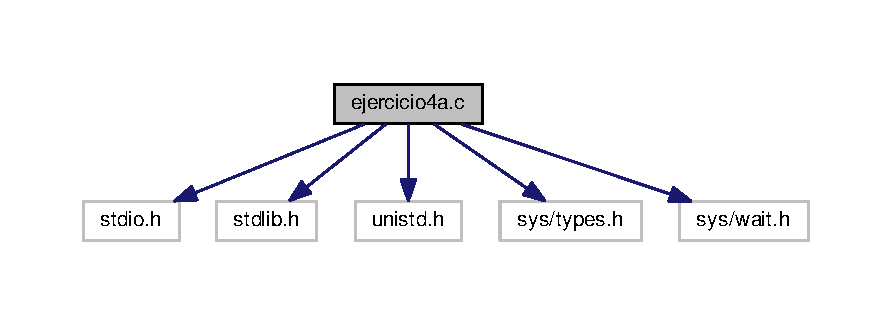
\includegraphics[width=350pt]{ejercicio4a_8c__incl}
\end{center}
\end{figure}
\subsection*{'defines'}
\begin{DoxyCompactItemize}
\item 
\hypertarget{ejercicio4a_8c_acee2369f62e4a096d243dec3cd7d0b00}{\#define {\bfseries N\+U\+M\+\_\+\+P\+R\+O\+C}~3}\label{ejercicio4a_8c_acee2369f62e4a096d243dec3cd7d0b00}

\end{DoxyCompactItemize}
\subsection*{Funciones}
\begin{DoxyCompactItemize}
\item 
\hypertarget{ejercicio4a_8c_a840291bc02cba5474a4cb46a9b9566fe}{int {\bfseries main} (void)}\label{ejercicio4a_8c_a840291bc02cba5474a4cb46a9b9566fe}

\end{DoxyCompactItemize}


\subsection{Descripción detallada}
Fuente del ejercicio 4. 

Este modulo hace una serie de forks e imprime los pid del padre y del hijo de cada uno de estos.

\begin{DoxyAuthor}{Autor}
Pareja 21\+: Juan Riera Gomez (\href{mailto:juan.riera@estudiante.uam.es}{\tt juan.\+riera@estudiante.\+uam.\+es}) y Carlos Ignacio Isasa Martín (\href{mailto:carlos.isasa@estudiante.uam.es}{\tt carlos.\+isasa@estudiante.\+uam.\+es}) 
\end{DoxyAuthor}
\begin{DoxyVersion}{Versión}
1.\+0 
\end{DoxyVersion}
\begin{DoxyDate}{Fecha}
02-\/03-\/2017 
\end{DoxyDate}

%--- End generated contents ---

% Index
\backmatter
\newpage
\phantomsection
\clearemptydoublepage
\addcontentsline{toc}{chapter}{Index}
\printindex

\end{document}
